%===================
% TODOs:
% Use metric unitis to specify coordinates (very important)
% Einzeilige Events, wenn Platz nicht reicht.

\documentclass[10pt,a4paper, landscape, ngerman]{article}
\usepackage[utf8]{inputenc}
\usepackage[left=2cm,right=2cm,top=2cm,bottom=2cm]{geometry}
\usepackage{babel}
\usepackage{translator}

\usepackage[T1]{fontenc}


\author{Tim Benedikt Herbstrith}
\pagestyle{empty}

\usepackage{tikz}
\usepackage{pgfcore}
\usepackage{pgfcalendar}


\usepackage{setspace}
\renewcommand{\arraystretch}{1.5}

\newcommand{\firstH}{11}
\newcommand{\lastH}{19}


% Macro for drawing calendar entries
\newcommand{\appointment}[5]{
	\filldraw[black!20, rounded corners] ({day(#1,-1)},{time(#2)}) rectangle ({day(#1,1)},{time(#3)});%
	\node[font=\scriptsize, text width=3cm] at ({day(#1,0)},{halftime(#2,#3)}) {#2\\ \textbf{#4}\\ #5};
%\path (#1-1,\firstH -#2) -- (#1,\firstH -#3) node[circle split,midway, font=\scriptsize, text width=3cm, minimum width=1, text centered] {#4 \nodepart{lower} #5};
}

\begin{document}
\begin{center}

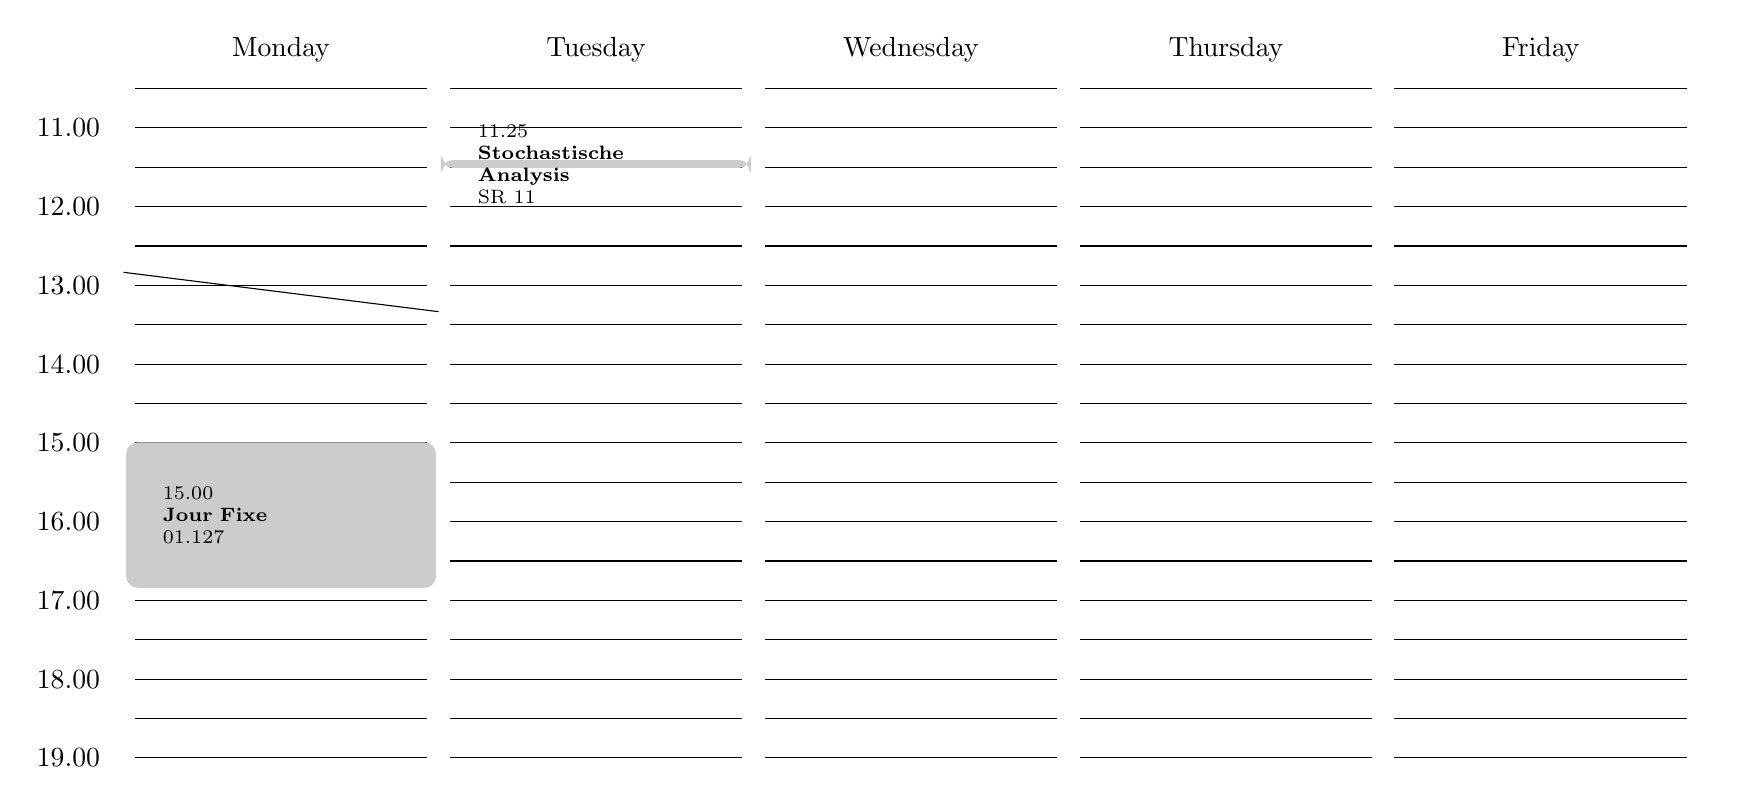
\begin{tikzpicture}[xscale=4, yscale=1]

% Offset for the rectangle marking appointments
\pgfmathsetmacro{\offsetForAppointment}{+0.01}

% Converts the integer marking the day of the week to a coordinate.
% The second argument specifies wheter the left (-1), the base (0) or the right end of the column is returned.
\pgfmathdeclarefunction{day}{2}{%
	\pgfmathparse{-#2*\offsetForAppointment+#1-(1-#2)/2}%
}

% Converts a given time (hh.mm) to a length. \firstH is converted to 0.
\pgfmathdeclarefunction{time}{1}{%
	\pgfmathparse{\firstH-(floor(#1)+(#1-floor(#1))/0.6)}%
}
\pgfmathdeclarefunction{halftime}{2}{%
	\pgfmathparse{(time(#1)+time(#2))/2}%
}
	
\foreach \hour in {\firstH,...,\lastH}
	\draw (0,\firstH-\hour) node[left=5] {\hour.00} -- (5,\firstH-\hour)  (0,\firstH+0.5-\hour) -- (5,\firstH+0.5-\hour);
\foreach \day in {0,...,5}
	\draw[line width=8pt,white] (\day,0.6) -- (\day,\firstH-\lastH -0.1);
\foreach \day in {0,...,4}
	\node at (0.5+\day,1) {\pgfcalendarweekdayname{\day}};
	
\appointment{1}{15.00}{16.50}{Jour Fixe}{01.127}
\appointment{2}{11.25}{11.30}{Stochastische Analysis}{SR 11}
%\appointment{3}{15.00}{16.50}{Hilfsmittel aus der EDV}{PC 02}
%\appointment{3}{17.25}{18.75}{Fragestunden}{HS 13}
%\appointment{4}{17.25}{18.75}{Fragestunden}{HS 13}
%\appointment{4}{11.25}{12.83}{Stochastische Analysis}{SR 08}

\draw (0,{time(12.50)}) -- (1cm,{time(13.20)});
\end{tikzpicture}

\end{center}
\end{document}